\documentclass[11pt]{article}

\usepackage[margin=1in]{geometry}
\usepackage{amsmath,amssymb}
\usepackage{booktabs}
\usepackage{graphicx}
\usepackage[colorlinks=true,linkcolor=blue,citecolor=blue,urlcolor=blue]{hyperref}
\usepackage{tikz}
\usetikzlibrary{positioning,arrows.meta,calc}

\newcommand{\eps}{\varepsilon}
\newcommand{\CA}{C_A}
\newcommand{\CF}{C_F}
\newcommand{\as}{\alpha_s}
\newcommand{\FF}{\mathbb{F}_p}

\title{A collinear-factorization workflow for the two-loop hard
functions of $pp \to h X$\\[1ex]
\large Method description of the \textsf{FeynFacet} pipeline}
\author{Max Zhang}
\date{\today}

\begin{document}
\maketitle

\begin{abstract}
We describe an automated workflow that computes next-to-next-to-leading
order (two-loop) partonic hard functions for single-inclusive hadron
production, $pp \to h X$, within collinear factorization at twist two,
for both unpolarized and polarized (including chiral-odd) channels.
The pipeline proceeds from process definitions to squared amplitudes
projected onto twist-two correlators, maps the real-emission phase-space
integrals to loop integrals by reverse unitarity, reduces them to master
integrals by integration-by-parts identities, and reconstructs the exact
rational master coefficients over finite fields.  Two methodological
elements are emphasized: a rationalization scheme that confines all
square-root kinematics to a transient, entry-local change of variables,
so that the finite-field probes run over the physical variables
$\{\CA,\CF,\eps,x,y\}$; and a decomposition of every coefficient into
classes of non-rational ``signatures,'' defined modulo the
multiplicative group of the rational function field, which keeps the
reconstruction problem minimal.  All stages are validated by exact
golden regressions at successively cheaper scales and by probe-count
parity with an independent earlier implementation.
\end{abstract}

\section{Introduction}

Single-inclusive hadron production, $p\,p \to h\,X$, is a classic
observable for the extraction of collinear parton distribution and
fragmentation functions, including the polarized and chiral-odd
distributions accessible with transversely polarized beams.  Extending
its theoretical description to next-to-next-to-leading order (NNLO)
requires the two-loop hard functions of all partonic channels: the
double-real, real-virtual, and double-virtual corrections to
$a\,b \to c\,X$, projected onto the twist-two collinear correlators of
the incoming hadrons and of the fragmenting parton.

This document describes the computational workflow we use to obtain
these hard functions, currently exercised in full on the double-real
contributions.  It is written as a method description rather than an
implementation record: the emphasis is on \emph{what} is computed at
each stage, in \emph{which} scheme, and \emph{why} the stages are
organized as they are.  The workflow is orchestrated by a
\textsc{Mathematica} package, \textsf{FeynFacet}, which drives the
established tool chain \textsf{FeynArts} (diagram generation),
\textsf{FeynCalc}/\textsf{FeynHelpers} (Dirac, color, and loop-integral
algebra), \textsf{Kira} (integration-by-parts reduction), and
\textsf{Ratracer}/\textsf{FireFly} (finite-field rational
reconstruction).

Section~\ref{sec:framework} fixes the theoretical framework.
Section~\ref{sec:workflow} walks through the pipeline stage by stage.
Section~\ref{sec:coefficients} describes the finite-field coefficient
reconstruction, which contains the main methodological novelties.
Section~\ref{sec:validation} summarizes the validation strategy, and
Section~\ref{sec:outlook} the remaining steps toward complete NNLO hard
functions.

\section{Theoretical framework}
\label{sec:framework}

\subsection{Collinear factorization at twist two}

At leading power in $\Lambda_{\rm QCD}/p_T$, the differential cross
section factorizes into convolutions of universal long-distance
functions with perturbative hard functions,
\begin{equation}
  d\sigma_{pp\to hX}
  \;=\;
  \sum_{a,b,c}\;
  f_a(x_a,\mu) \,\otimes\, f_b(x_b,\mu) \,\otimes\,
  D_{h/c}(z_h,\mu) \,\otimes\,
  \hat\omega_{ab\to c}\!\left(x,y;\as(\mu),\eps\right),
  \label{eq:fact}
\end{equation}
where $x_{a,b}$ are the light-cone momentum fractions of the incoming
partons, $z_h$ that of the observed hadron relative to the fragmenting
parton $c$, and the hard functions $\hat\omega$ depend on the partonic
Mandelstam ratios
\begin{equation}
  x = -\,\frac{t}{s}, \qquad y = -\,\frac{u}{s},
  \qquad 0 < x,\; 0 < y,\; x+y < 1 .
\end{equation}
The long-distance functions are the twist-two collinear correlators:
for the incoming protons the unpolarized, helicity, and transversity
distributions $f_1$, $g_{1L}$, $h_1$; for the fragmenting parton the
corresponding fragmentation correlators $D_1$, $G_{1L}$, $H_1$.  Each
polarization channel (e.g.\ the unpolarized channel $UU$, the
double-transverse channel $TT$) selects a definite set of correlators
and a definite Dirac/Lorentz projection of the partonic amplitude.

\subsection{Regularization scheme}

All partonic computations are performed in dimensional regularization
with $d = 4 - 2\eps$ in the
Breitenlohner--Maison--'t\,Hooft--Veltman (BMHV) scheme for $\gamma_5$.
The chiral-odd channels then require careful bookkeeping of evanescent
structures: transverse-polarization projections generate evanescent
scalar products (the $(-2\eps)$-dimensional components of transverse
vectors), which are retained exactly as additional variables through
the reduction and only combined at the level of the finite hard
functions.  Dimensional-shift (Tarasov) identities are used where the
tensor/dimension bookkeeping of the projected integrands calls for
them; the scheme dependence introduced at intermediate stages is
validated by the exact regression tests of
Section~\ref{sec:validation}.

\subsection{Reverse unitarity}

The double-real hard functions are phase-space integrals of squared
amplitudes.  We map them to two-loop integrals by reverse unitarity:
each on-shell delta function is replaced by a cut propagator,
\begin{equation}
  \delta^{(+)}\!\left(p^2\right)
  \;\longrightarrow\;
  \frac{1}{2\pi i}
  \left[
    \frac{1}{p^2 + i0} - \frac{1}{p^2 - i0}
  \right],
\end{equation}
after which the integrals obey integration-by-parts identities in
which any sector with a vanished cut propagator is set to zero.  The
phase-space measure, the flux, and the convolution variables of
Eq.~\eqref{eq:fact} are carried along exactly, including the endpoint
(plus-distribution) structure in the momentum fractions, which is kept
symbolic through a declared distributional prefactor rather than being
expanded prematurely.

\section{The workflow}
\label{sec:workflow}

The pipeline consists of the stages summarized in
Fig.~\ref{fig:flow-long}; each stage writes a fingerprinted artifact
that the next stage validates on load, so that any stage can be re-run
or resumed independently.

\begin{figure}[t]
\centering
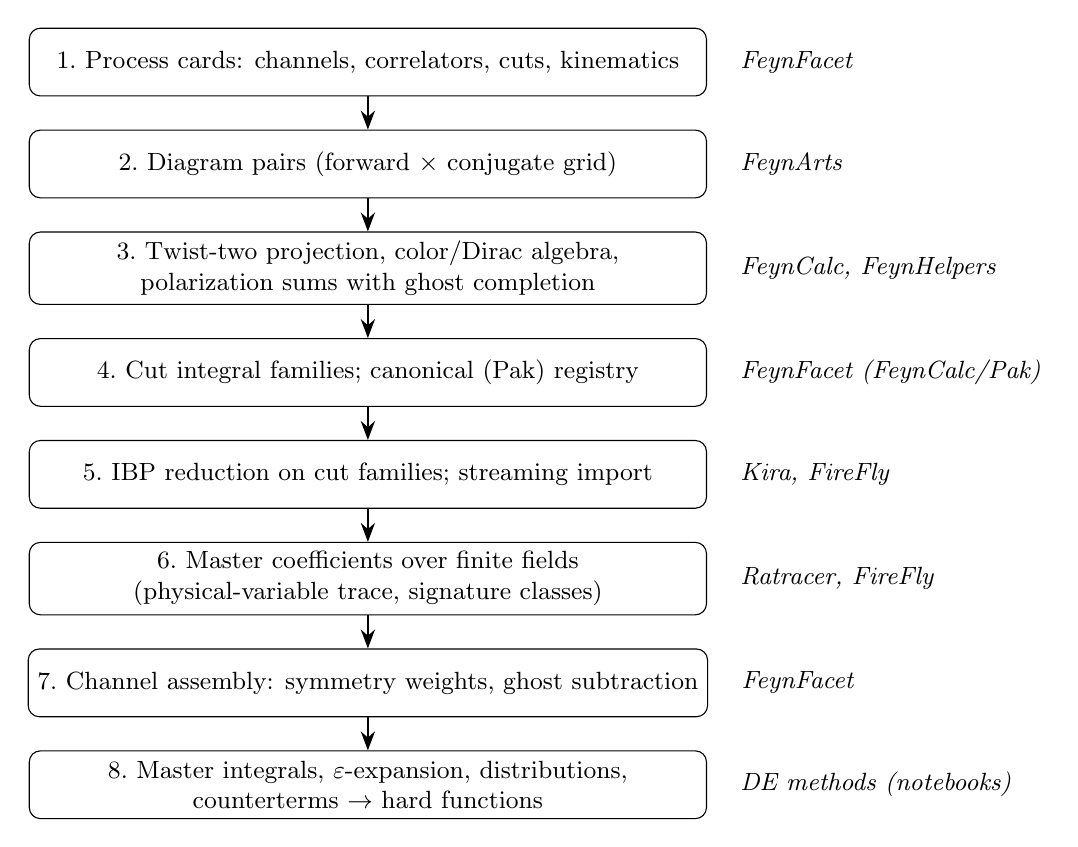
\begin{tikzpicture}[
  stage/.style={draw, rounded corners, align=center, minimum width=8.6cm,
    minimum height=0.86cm, font=\small},
  tool/.style={font=\small\itshape, anchor=west},
  arrow/.style={-{Stealth[length=2.4mm]}, thick},
  node distance=0.42cm
]
\node[stage] (cards) {1.\ Process cards: channels, correlators, cuts,
kinematics};
\node[stage, below=of cards] (diagrams) {2.\ Diagram pairs
(forward $\times$ conjugate grid)};
\node[stage, below=of diagrams] (project) {3.\ Twist-two projection,
color/Dirac algebra,\\ polarization sums with ghost completion};
\node[stage, below=of project] (families) {4.\ Cut integral families;
canonical (Pak) registry};
\node[stage, below=of families] (ibp) {5.\ IBP reduction on cut
families; streaming import};
\node[stage, below=of ibp] (coeff) {6.\ Master coefficients over
finite fields\\ (physical-variable trace, signature classes)};
\node[stage, below=of coeff] (assembly) {7.\ Channel assembly:
symmetry weights, ghost subtraction};
\node[stage, below=of assembly] (masters) {8.\ Master integrals,
$\eps$-expansion, distributions,\\ counterterms $\to$ hard functions};
\foreach \a/\b in {cards/diagrams, diagrams/project, project/families,
  families/ibp, ibp/coeff, coeff/assembly, assembly/masters}
  \draw[arrow] (\a) -- (\b);
\node[tool] at ($(cards.east)+(0.3,0)$) {FeynFacet};
\node[tool] at ($(diagrams.east)+(0.3,0)$) {FeynArts};
\node[tool] at ($(project.east)+(0.3,0)$) {FeynCalc, FeynHelpers};
\node[tool] at ($(families.east)+(0.3,0)$) {FeynFacet (FeynCalc/Pak)};
\node[tool] at ($(ibp.east)+(0.3,0)$) {Kira, FireFly};
\node[tool] at ($(coeff.east)+(0.3,0)$) {Ratracer, FireFly};
\node[tool] at ($(assembly.east)+(0.3,0)$) {FeynFacet};
\node[tool] at ($(masters.east)+(0.3,0)$) {DE methods (notebooks)};
\end{tikzpicture}
\caption{The stages of the workflow and the principal tool used at each
stage.  Every stage is driven by \textsf{FeynFacet}, which owns the
artifact formats and validation.}
\label{fig:flow-long}
\end{figure}

\subsection{Process cards}

A \emph{card} declares one partonic channel of one polarization
configuration: the external states and their untagged/tagged status,
the correlators to project onto, the cut structure, the declared
distributional prefactor (e.g.\
$f_1(x_a)\,f_1(x_b)\,D_1(z_h)$ with its Laurent valuations in the
endpoint variables), the kinematic scale and mass dimensions, the
dimensionless coordinates $(x,y)$, and the physical region.  Cards are
purely declarative; every later stage reads its conventions from the
card, so a polarization channel is added without touching the pipeline.

\subsection{Diagram pairs}

Feynman diagrams for the forward amplitude and its conjugate are
generated with \textsf{FeynArts}.  The squared amplitude is organized
as the full forward~$\times$~conjugate grid of diagram pairs (at NNLO
double-real, $36 \times 36$ pairs per channel); each pair is an
independent unit of work, which makes the stage embarrassingly
parallel and restartable at pair granularity.

\subsection{Projection and gauge completion}

Each pair is contracted with the twist-two projectors of its channel
and reduced by Dirac and color algebra
(\textsf{FeynCalc}/\textsf{FeynHelpers}) to a scalar integrand on the
cut.  Two points deserve emphasis:

\paragraph{Ghost completion of gluon polarization sums.}  For final
states with a pair of cut gluons, the polarization sums are performed
with the Feynman-gauge metric ($-g^{\mu\nu}$), and the unphysical
polarizations are removed by the Slavnov--Taylor completion: a
companion channel with a cut ghost--antighost pair is computed through
the \emph{identical} pipeline, and the physical result is assembled as
\begin{equation}
  \sigma_{gg}
  \;=\;
  \frac{1}{2!}\;\sigma^{(-g)}_{\text{gluon pair}}
  \;-\;
  \sigma_{\text{ghost pair}} ,
  \label{eq:ghost}
\end{equation}
where $1/2!$ is the identical-particle factor of the two untagged
gluons.  Both terms are two-loop cut integrals; no additional loop
order is introduced.  Light-cone axial gauges for the polarization sum
were considered and rejected: the axial denominators would contaminate
the integral families and the subsequent basis construction.

\paragraph{Identical-particle weights.}  The phase-space symmetry
factor $1/n!$ per species of $n$ identical untagged final-state
partons is derived from the card and applied once, at the assembly
stage, together with the sign of Eq.~\eqref{eq:ghost}.

\subsection{Canonical cut families}
\label{sec:families}

The scalar integrands populate integral \emph{families}: sets of
propagators (including the cut ones) closed under the IBP operations.
Families arising from different pairs are recognized as equivalent by
a cut-aware canonicalization based on the Pak algorithm: cut
propagators are marked by auxiliary masses so that the canonical form
distinguishes cut from uncut lines, and momentum shifts identified on
the canonical form are verified exactly.  Equivalent families are
merged into a global registry with stable, cross-run family names;
registries of related channels (e.g.\ the gluon and ghost grids of
Eq.~\eqref{eq:ghost}) are seeded from one another so that both
channels live in a single family namespace and can be assembled
integral by integral.  At NNLO double-real this merges $1898$ raw
sectors into $430$ canonical families, of which $374$ carry reduction
targets.

\subsection{IBP reduction}

The reduction to master integrals is performed by \textsf{Kira} (with
\textsf{FireFly} as its finite-field backend), with the cut
propagators declared so that sectors with vanished cuts are dropped.
The solved system is imported family by family into a record-store
artifact: reduction tables are streamed to disk one family at a time
and closed transitively against the frontier of masters, so that the
peak memory of the import stage is set by the largest single family
rather than by the full system.  At NNLO double-real the reduction
maps $44\,877$ target integrals onto $347$ master integrals.

\subsection{Master coefficients over finite fields}

The IBP stage leaves every channel written as
\begin{equation}
  \hat\omega \;=\; \sum_{I \in \text{masters}} c_I \, \mathcal{M}_I ,
  \qquad
  c_I = c_I(\CA,\CF;\eps;x,y;\ldots),
\end{equation}
and the coefficients $c_I$ --- rational functions assembled from tens
of thousands of reduction entries --- are the practical bottleneck.
They are reconstructed exactly over finite fields; the method is
described in Section~\ref{sec:coefficients}.

\subsection{Assembly}

The assembly stage combines the per-channel coefficient sets with
their weights --- the identical-particle factor and the ghost
subtraction of Eq.~\eqref{eq:ghost} --- by merging master-by-master in
the shared canonical namespace of Section~\ref{sec:families}.  The
stage is fail-closed: namespace or phase-space-measure mismatches
between the channels abort the assembly rather than silently mixing
conventions.

\subsection{Downstream: masters and distributions}

The remaining analytic steps --- evaluation of the master integrals
(differential equations in $(x,y)$, canonical bases), expansion in
$\eps$, extraction of the endpoint plus-distributions against the
declared distributional prefactor, and mass-factorization
counterterms --- are performed outside the package in notebook
workflows, following the conventions fixed by the cards.  They are the
final stage toward the renormalized hard functions and are not further
described here.

\section{Finite-field reconstruction of the master coefficients}
\label{sec:coefficients}

The coefficient stage determines, for each master integral, one exact
rational function.  Symbolic simplification of the assembled
coefficients is hopeless at this size; instead the coefficients are
evaluated modularly and reconstructed.  Three design decisions make
this efficient.

\subsection{Physical variables only: transient rationalization}
\label{sec:rationalization}

After the hadronic substitution and division by the declared
distributional prefactor, individual contributions contain
half-integer powers of monomials in the momentum fractions and
invariants (a collinear-kinematics artifact).  A change of variables
$x_a = \xi_a^2$, $x_b = \xi_b^2$, $s = 2q^2$, \dots\ rationalizes
them, but performing the reconstruction \emph{in} the square-root
variables doubles the polynomial degrees seen by the reconstruction
and is prohibitively expensive.  Both problems are avoided by making
the rationalization \emph{entry-local and transient}:

\begin{enumerate}
\item Each additive contribution is lifted to the square-root
  variables, divided by the (trivially rationalized) prefactor, and
  canceled --- a small, bounded operation per entry.
\item Each entry is then \emph{descended} back to the invariants.
  Writing the entry as $N/D$ with
  $N = N_e + r\,N_o$, $D = D_e + r\,D_o$ (even/odd parts in a root
  variable $r$), the branch flip $r \to -r$ leaves the value invariant
  exactly when $N_e D_o - N_o D_e = 0$, and then
  $N/D = N_e/D_e$ identically.  The zero test runs on the small
  even/odd combination only; entries already even are restored
  structurally with no rational algebra at all.  Entries that fail
  individually are retried in same-denominator groups and, finally,
  as a single remainder; a survivor is a hard, labeled failure ---
  by measurement, none occurs in the physical channels.
\item The declared scale and $\as$ leave the rational part through
  exact mass-dimension homogeneity (their powers are read off
  structurally per entry), so the functions that reach the
  reconstruction depend on the physical variables
  $\{\CA, \CF, \eps, x, y\}$ only.
\end{enumerate}

Root-freeness of the final coefficients is certified after
reconstruction, on the small reconstructed objects, not on the large
inputs.

\subsection{Signature classes modulo the rational function field}
\label{sec:signatures}

The normalized entries are not globally rational: they carry exact
non-rational factors --- powers like $2^{\,m+n\eps}$ from the scale
map, residual constant roots such as $\sqrt2$, and, in chiral-odd
channels, evanescent structures.  Every entry is therefore split as
\begin{equation}
  \text{entry} \;=\; S \times R,
  \qquad
  R \in \mathbb{Q}(\CA,\CF,\eps,x,y),
\end{equation}
with the \emph{signature} $S$ collecting the non-rational factors, and
the coefficient of each master is stored as a small set of signature
classes, each with one rational function to reconstruct.

The essential point is the equivalence relation: signatures are
identified \emph{modulo the multiplicative group}
$\mathbb{Q}(\CA,\CF,\eps,x,y)^\times$.  Any factor of a signature that
is itself rational in the reconstruction variables is folded into the
rational part; for rational bases this is implemented by prime
decomposition,
\begin{equation}
  b^{\,m+n\eps} \;=\;
  \underbrace{\;b^{\,m}\;}_{\to\;R}
  \times
  \underbrace{\left(b^{\eps}\right)^{n}}_{\to\;S},
  \qquad
  b \;=\; \textstyle\prod_i p_i^{a_i},
\end{equation}
with a canonical representative per class.  Without this quotient the
classes fragment (the same rational function stored a dozen times,
differing by factors $2^k$), and the number of reconstruction probes
multiplies accordingly; with it, each master of the unpolarized NNLO
double-real channel carries exactly one class per power of the scale.
The scale and $\as$ monomials deliberately live in the signature, so
the per-master scale power remains an exactly readable property of the
stored artifact.

\subsection{Trace evaluation and rational reconstruction}

For each master, the surviving rational function is presented as a
plus-concatenation of its (entry-wise normalized and compacted)
contributions.  \textsf{Ratracer} compiles this input into an
arithmetic trace --- constant propagation, dead-code and
common-subexpression elimination --- and evaluates it over $63$-bit
prime fields; \textsf{FireFly} performs the multivariate rational
reconstruction from these probes.  Two practical observations govern
the cost:
\begin{itemize}
\item the \emph{probe count} is intrinsic: it is set by the true
  degrees and term counts of the reconstructed function (for the
  hardest columns, numerator degrees above $100$), and is minimized by
  the class quotient of Section~\ref{sec:signatures};
\item the \emph{probe time} is representational: it scales linearly
  with the compiled trace size, i.e.\ with the compactness of the
  input.  Entry-wise exact cancellation of each contribution (a
  bounded operation, performed in parallel) shrinks the largest
  columns by factors of $5$--$30$ and the probe time with them.
\end{itemize}
The columns of a channel share one trace, so common subexpressions
across masters are probed once; the largest columns can also be
reconstructed standalone when their probe requirements dominate.

\section{Validation}
\label{sec:validation}

The workflow is validated by exact, not numerical, comparisons, at the
cheapest scale that exercises each property:

\begin{itemize}
\item \textbf{Golden regressions.}  The NLO channel, the chiral-odd
  (transversity) NLO channel, and the NNLO ghost channel each have a
  stored reference result; the pipeline must reproduce them
  \emph{exactly} --- identical master sets and exactly equal
  coefficients --- after every methodological change.  These three
  references cover, respectively, the baseline pipeline, the
  evanescent/BMHV structures, and the full NNLO kinematics at small
  size.
\item \textbf{Sign-definiteness certificates.}  The positivity
  assumptions used by the rationalization of
  Section~\ref{sec:rationalization} rest on exact bounds for sums of
  massless invariants over the cut phase space, proved by a
  max-flow/min-cut convex-decomposition argument and cross-checked
  numerically on random phase-space points.
\item \textbf{Cross-implementation parity.}  For a benchmark master of
  the NNLO double-real channel, the reconstruction was compared
  against an independent earlier implementation of the same physics:
  both require the same number of finite-field probes (169.6k
  vs.\ 169.7k) and agree at matched wall time, confirming that the
  reconstructed functions and the input compactness are equivalent.
\item \textbf{Scheme checks.}  The BMHV dimensional-shift treatment
  was verified to be representation-only for the unpolarized channel
  (exactly zero integrand difference pair by pair against the
  pre-correction data), isolating its physical effect to the
  polarized channels, where the golden regression covers it.
\end{itemize}

A gauge/known-result check of the assembled $\sigma_{gg}$ combination
at a numerical phase-space point is scheduled once the full gluon-grid
coefficients are available.

\section{Status and outlook}
\label{sec:outlook}

The pipeline is complete and validated through the coefficient stage
for the unpolarized NNLO double-real channel: pair generation,
canonicalization ($430$ families), reduction ($44\,877$ targets,
$347$ masters), and the finite-field trace in physical variables with
canonical signature classes (one coefficient column per master).  The
ghost companion channel is fully reconstructed ($27$ masters in the
shared namespace), so the assembly of Eq.~\eqref{eq:ghost} is a single
step once the gluon-grid reconstruction is run.  The remaining NNLO
ingredients --- real-virtual and double-virtual channels --- reuse the
same stages with one-loop$\times$one-loop and two-loop virtual
integrands, and the downstream master-integral and distribution
expansion completes the hard functions.

\vspace{2ex}
\noindent\textbf{Tool summary.}
\textsf{FeynArts} (diagrams);
\textsf{FeynCalc} + \textsf{FeynHelpers} (projection and algebra, Pak
canonical forms);
\textsf{Kira} + \textsf{FireFly} (IBP reduction on cut families);
\textsf{Ratracer} + \textsf{FireFly} (arithmetic traces and rational
reconstruction);
\textsf{FeynFacet} (orchestration, cards, family registry, streaming
artifacts, signature classes, assembly, regression harness);
\textsc{Mathematica} throughout.

\end{document}
